\documentclass[Main.tex]{subfiles}
\begin{document}
\section{Introduction}
Over the past two decades the field of swarm intelligence has evolved from intertwined branches of mathematics, physics, biology, traditional robotics, and artificial intelligence; attempting to apply observations of physical and biological systems to artificial ones. This has led to novel approaches in the design and analysis of multi-agent systems and the algorithms associated with them. It has spawned an entirely new field of research called \emph{swarm robotics}\citep{Sahin2005}, which has led to a large number of platforms, algorithms, and analyis tools \citep{Bramiblla2013}.

This survey paper attempts to collate the research focusing on mathematical and computational modeling techniques that have been developed to help describe the temporal and spatial evolution of a swarm of robots programmed to perform specific, collaborative tasks. In particular, we describe the evolution of the field since \possessivecite{Lerman2005} review, including recent work on spatial modeling techniques building up on Langevin and Fokker-Planck equations, as well as on model-based optimization.

Swarm systems have many benefits over traditional, centralized robot systems. The robots used in swarm applications are generally many orders of magnitude smaller (centimeters vs.\ meters, grams vs.\ kilograms) and simpler in design ($<10$ actuators vs. $100$s of actuators) than conventional robots. Also, most swarm systems are homogeneous---robots with identical software/hardware are used to complete the assigned task. This makes swarm systems easily scalable while simultaneously keeping manufacturing and maintenance costs of the hardware low. Though, perhaps their greatest advantage is system stability and robustness to error. Most swarm systems consist of small, relatively simple robots that are only capable of limited and noisy sensing, communication and actuation. This means that while no single robot alone is capable of performing the task assigned, the system as a whole is resilient to individual errors from agents and is capable of completing the task \cite{Winfield2005}.

\begin{figure}[!ht]
\centering\begin{subfigure}{.5\textwidth}
\centering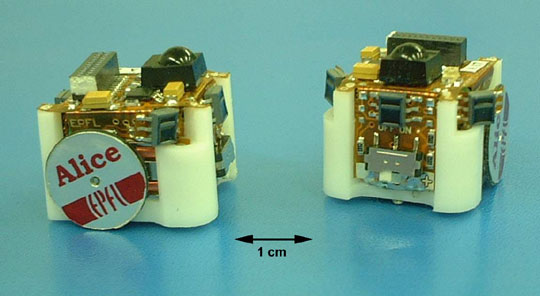
\includegraphics[height=4cm,width=6.5cm]{assets/alicerobot.png}
\caption{Alice robot}
\end{subfigure}~
\centering\begin{subfigure}{.5\textwidth}
\centering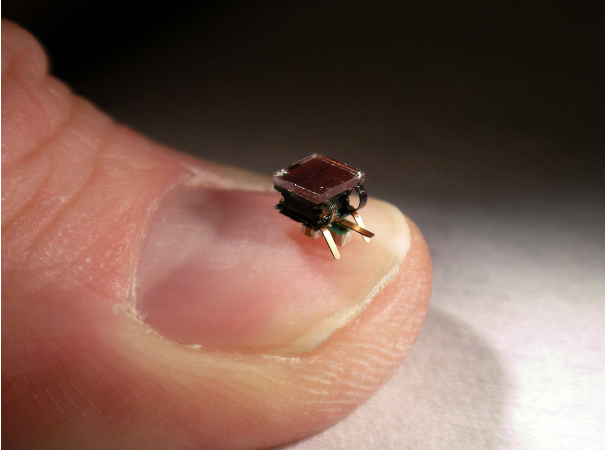
\includegraphics[height=4cm,width=6.5cm]{assets/iswarm.png}
\caption{I-SWARM robot concept}
\end{subfigure}\vspace{1cm}
\centering\begin{subfigure}{.5\textwidth}
\centering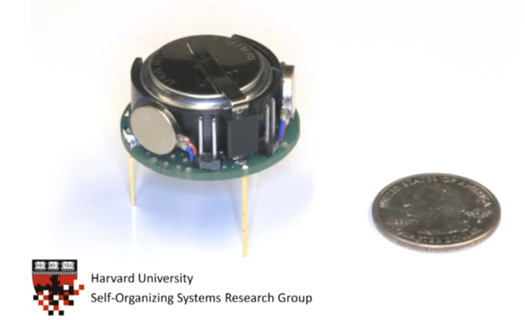
\includegraphics[height=4cm,width=6.5cm]{assets/kilobotrobot.png}
\caption{Kilobot robot}
\end{subfigure}~
\centering\begin{subfigure}{.5\textwidth}
\centering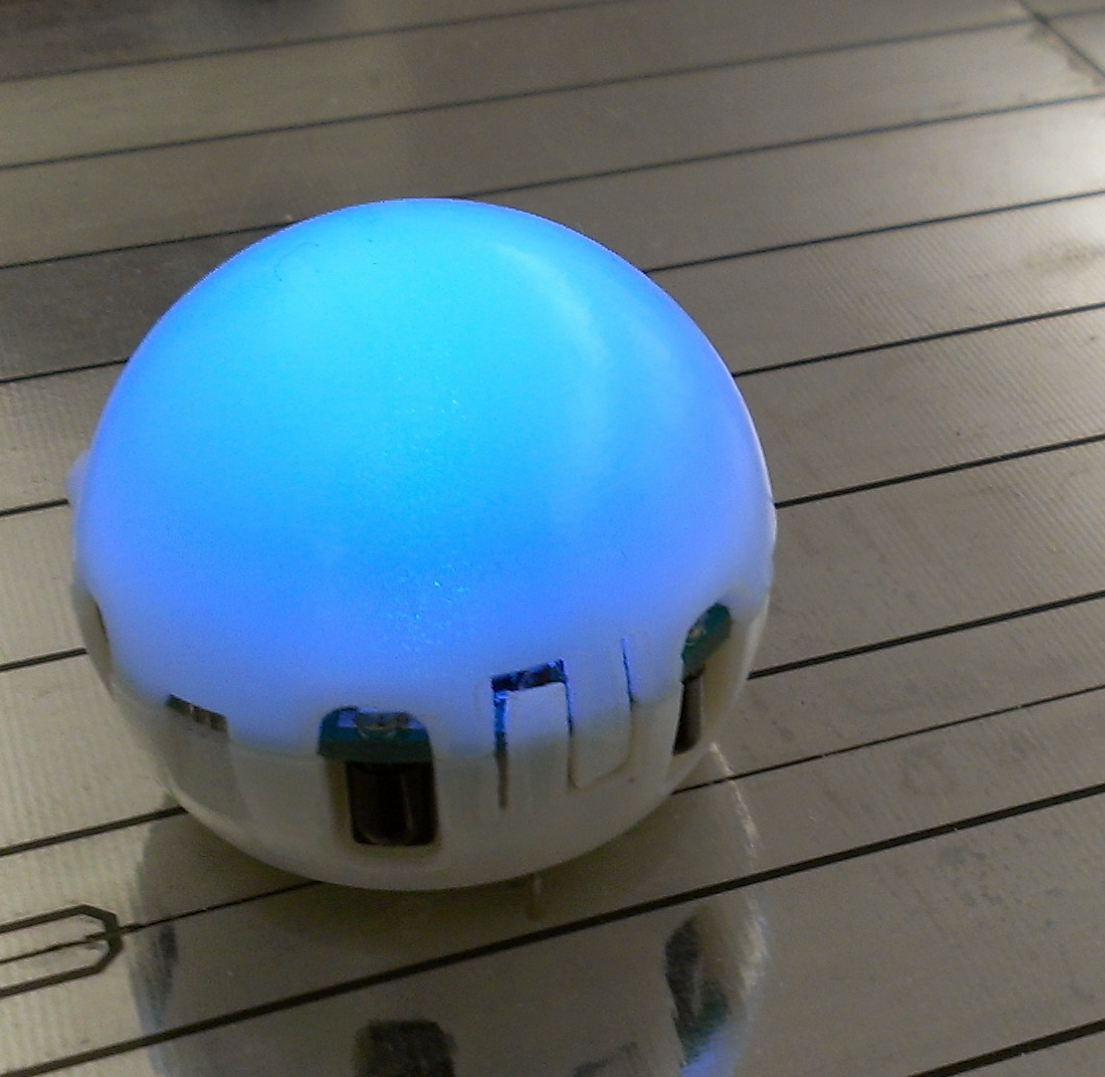
\includegraphics[height=4cm,width=5cm]{assets/dropletrobot.png}
\caption{Droplet robot}
\end{subfigure}
\caption{Clock-wise from the top left: The Alice robot \citep{caprari2005mobile}\label{fig:swarmbots}, the i-Swarm platform \citep{Seyfried2005}, the kilobot \citep{Rubenstein2012}, and the Droplet \cite{farrow14}}
\end{figure}

In order to make swarms an alternative engineering approach---in which robustness emerges despite predictable, indivdiual failure---we require formal tools that allow us to predict and verify the resulting complex behavior. Developing such tools goes hand-in-hand with investigating novel hardware (Figure \ref{fig:swarmbots}), simulation tools \citep{Michel1998}, and tracking 
tools \cite{correlliros06,lochmatter08} that ease conducting large number of experiments with large number of robots, as they allow analyzing swarm dynamics on a higher abstraction level. This not only allows to explore the design space much faster, but also to use analyis and numerical methods for optimization and verification. 


%Methods for modeling a swarm system are therefore extremely important as they provide a formal understanding of the relationship between control parameters, physical properties, and performance. These models can then be used to provide formal guarantees on performance as well as system identification and parameter optimization\citep{Correll2006a,Correll2008}.

With this motivation for modeling swarm systems in mind, the rest of the paper is structured as follows. The next section describes and defines the technical terms that will be used for the remainder of this paper. While many of the terms, such as, spatial, non-spatial, robot, etc. can have very broad and general definitions, this section aims to define them more specifically in the context of this survey paper. Section \ref{sec:methods} outlines a general methodology often used in the swarm robotics community for designing and optimizing a robot controllers and developing swarm system models. Section \ref{sec:nonspatial} covers non-spatial modeling applications using an array of well known swarm robot experiments. The end of this section also describes original work done in designing a novel robot controller for multi-robot collaboration based on a sigmoid threshold response function. In the proceeding section we begin to explore the relatively new direction of spatial models in swarm robotics. The models discussed in this section are heavily inspired by physical models of Brownian motion and involve the use of the Langevin equation and the Fokker--Planck equation. Finally, the conclusion provides a short summary of open questions in the field of swarm system modeling and open research problems.
\end{document} 